\section{Scelte implementative}
\label{cap:implementation-choices}

\subsection{Codice templatizzato}

Al fine di rendere il codice quanto più generico ed estendibile, molte delle classi e dei metodi scritti
usano i template C++, corrispondenti ai generics in Java.
I nomi ricorrenti dei tipi generici impiegati sono \codeinline{Label} e \codeinline{Weight}.
\codeinline{Label} denota il tipo del nome di un nodo del grafo. È istanziato come \codeinline{size\_t}, corrispondente a \codeinline{unsigned long long}, occupa almeno 64bit può rappresentare solo valori $\geq 0$.
\codeinline{Weight} denota il tipo del peso di un arco del grafo. È istanziato come \codeinline{long}, corrispondente a \codeinline{signed long int},
occupa almeno 32bit.

\subsection{Rappresentazione del grafo}
\label{sub:graph-representation}

Gli algoritmi di questo homework operano su grafi pesati connessi e non diretti.
Le operazioni sui grafi di cui abbiamo bisogno sono:

\begin{itemize}
    \item Creazione di un grafo a partire da una lista di archi in input, con ($n$) vertici e ($m$) archi noti a priori, e con nodi etichettati nell'intervallo $ [0, n-1] $ ;
    \item Enumerazione degli archi del grafo;
    \item Enumerazione dei vertici del grafo;
    \item Ottenere dei vertici adiacenti ad un nodo;
    \item Enumerazione dei vertici adiacenti ad un nodo;
    \item Aggiunta di un arco (escludendo archi duplicati di peso non minimo);
    \item Rimozione di un arco.
\end{itemize}

\noindent Le due rappresentazioni più comuni per rappresentare un grafo sono \textbf{Matrici di Adiacenza} (\textit{Adj. Matrix}) o \textbf{Liste di Adiacenza} (\textit{Adj. List}). L'utilizzo di Matrici di Adiacenza è solitamente giustificato da grafi molto densi (non è il nostro caso, visto che il numero di archi è sempre molto vicino al numero di nodi). Per grafi sparsi, le Liste di Adiacenza sono una buona scelta di default. \\

\noindent Noi abbiamo deciso invece di utilizzare una \textbf{Mappa di Adiacenza} (\textit{Adj. Map}), la quale ci permette complessità temporali migliori per le operazioni richieste a scapito di un moderato aumento della complessità spaziale, che rimane comunque \complexityNPlusM{}, lo stesso delle Matrici di Adiacenza. Nella tabella \ref{table:graph-representation-comparison} è possibile vedere un confronto tra le 3 diverse rappresentazioni di grafi possibili citate sopra. \\

\noindent L'occupazione di spazio aggiuntiva è dovuta all'utilizzo di una \codeinline{std::unordered\_map} e un \newline \codeinline{std::unordered\_set} ausiliario. Quest'ultimo tiene traccia degli archi inseriti per permettere una rapida estrazione, modifica e cancellazione degli archi del grafo. La mappa è invece usata per mappare ogni nodo ad un'altra mappa (nodo $\rightarrow{}$ peso), usata per eliminare efficacemente i nodi duplicati di peso non minimo al momento della creazione del grafo (scelta necessaria, vista la presenza di archi duplicati nei dataset dati). L'uso di mappe ci permette inoltre di individuare ed eliminare archi in tempo \complexityConstant{} ammortizzato.

\begin{table}[ht]
\centering
    \begin{tabular}{|l|ccc|}
    \hline
    &  \multicolumn{1}{c}{Adj. Matrix} & \multicolumn{1}{c}{Adj. List} & \multicolumn{1}{c|}{Adj. Map} \\
    \hline
     Complessità spaziale   & \complexityNSquared{}  & \complexityNPlusM{} & \complexityNPlusM{} \\ \hline

     Creazione grafo & \complexityNSquared{}  & \complexityNPlusM{} & \complexityNPlusM{} \\
     Enumerazione archi & \complexityNSquared{} & \complexityM{} & \complexityM{} \\
     Enumerazione vertici & \complexityN{} & \complexityN{} & \complexityN{} \\
     Ottenere vertici adiacenti ad un nodo & \complexityN{} & \complexityNDegree{} & \complexityConstant{} \\
     Enumerazione vertici adiacenti ad un nodo & \complexityN{} & \complexityNDegree{} &  \complexityNDegree{} \\
     Aggiunta arco & \complexityConstant{} & \complexityConstant{} & \complexityConstant{} \\
     Rimozione arco & \complexityConstant{} & \complexityM{} & \complexityConstant{} \\
    \hline
    \end{tabular}
    \caption{Confronto di complessità spaziali (prima riga) e complessità temporali di alcune operazioni su grafi rappresentati da diverse strutture dati.}
    \label{table:graph-representation-comparison}
\end{table}

\noindent Il diagramma di classe in figura \ref{fig:AdjMapGraph Class} riporta gli attributi e i metodi offerti dalla classe AdjacentMapGraph.

\begin{figure}[h]
	\caption{Diagramma di classe per AdjacentMapGraph, definita in \codeinline{Shared/AdjacentMapGraph.h}}
	\centering
	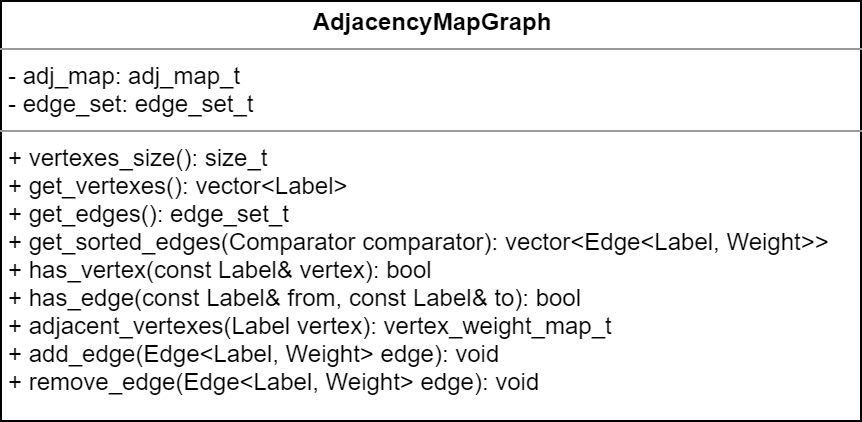
\includegraphics[width=0.7\textwidth]{./images/AdjancencyMapGrapClass.png}
	\label{fig:AdjMapGraph Class}
\end{figure}

\noindent In figura \ref{fig:AdjMapGraph Abstract} è illustrato un esempio di trasformazione di un grafo in mappa di adiacenza. Si può notare che la mappa di adiacenza è composta da una prima mappa avente una chiave per ogni vertice del grafo (\codeinline{adj\_map\_t}). Ogni entry della mappa è composta dalla chiave che rappresenta il nome del nodo e da un valore che associa al nodo un'altra mappa (\codeinline{vertex\_weight\_map\_t}), che rappresenta gli archi del grafo.
In particolare, \codeinline{vertex\_weight\_map\_t} ha come chiave l'etichetta del vertice opposto, e come valore il peso dell'arco dal vertice di origine. \\

\noindent Quindi, tutte le operazioni di inserimento, ricerca, cancellazione e aggiornamento sono eseguite in tempo costante ammortizzato. Gli unici aspetti negativi sono un'occupazione di spazio più grande di un fattore costante (ma sempre \complexityNPlusM{}) e una maggiore complessità nel mantenere le strutture dati ausiliarie sempre aggiornate. Poiché i grafi del dataset assegnato occupano una porzione minima di memoria, riteniamo questi tradeoff accettabili. \\

\begin{figure}[h]
	\caption{Rappresentazione della mappa di adiacenza}
	\centering
	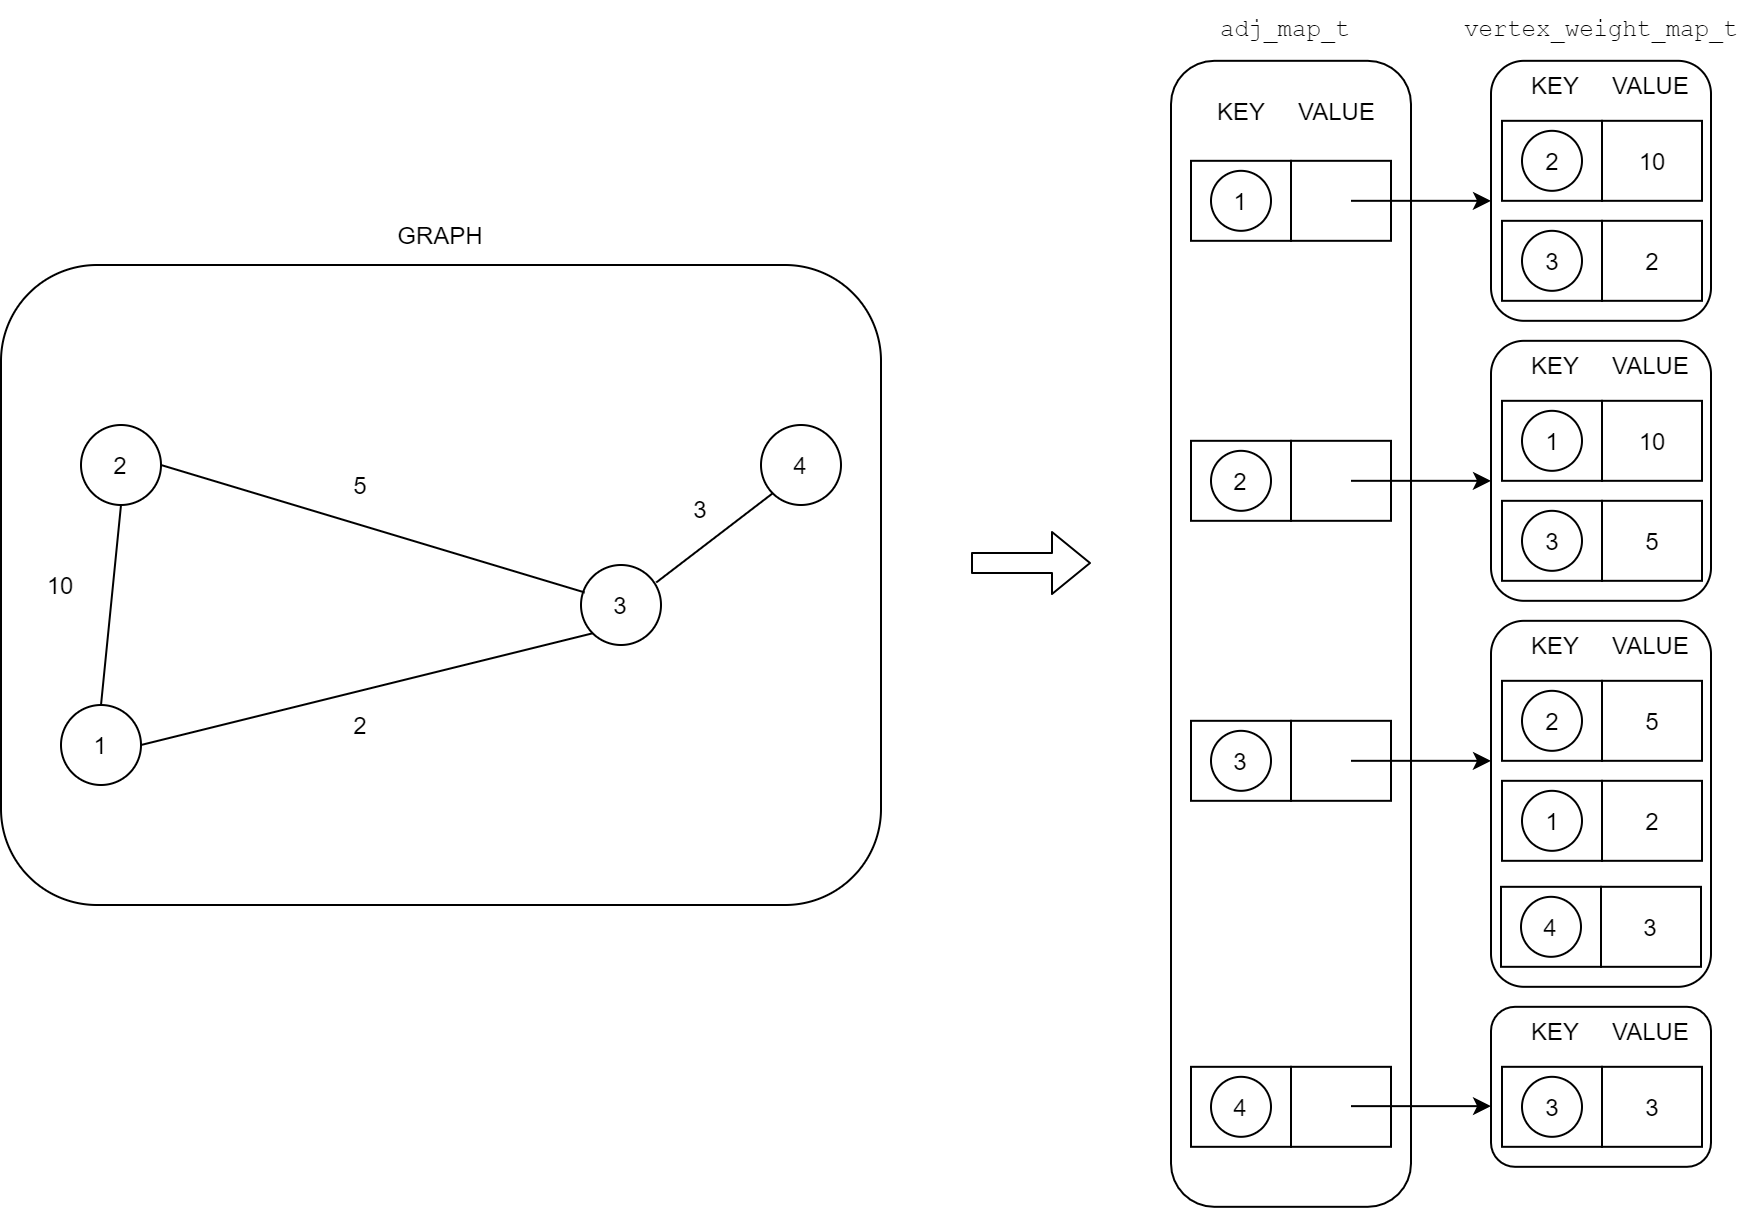
\includegraphics[width=0.7\textwidth]{./images/AdjMapGraphAbstract.png}
	\label{fig:AdjMapGraph Abstract}
\end{figure}

\noindent Il campo \codeinline{adj\_map} permette quindi di rappresentare un grafo non diretto pesato, ma da solo non basta ad ottenere le complessità temporali che ci eravamo prefissati. In particolare, l'utilizzo di un container \textit{std::unordered\_set} ausiliario ha i seguenti vantaggi:

\begin{itemize}
    \item Rende \complexityConstant{} la complessità temporale del metodo \codeinline{get\_edges()}, evitando la scansione dell'intera mappa di adiacenza per ricavare la lista degli archi ad ogni step della scansione. Quet'ultima scansione avrebbe un'ulteriore problema: se ad esempio sussiste un arco tra i vertici 2 e 3 (come nell'esempio in figura \ref{fig:AdjMapGraph Abstract}), nella lista di archi verrebbe ritornato sia l'arco $2 \rightarrow 3$ che $3 \rightarrow 2$;
    \item Se opportunamente configurato, ci permette di garantire l'assenza di archi doppi (come quelli visti nell'esempio precedente, $2 \rightarrow 3$ e $3 \rightarrow 2$). Per ottenere ciò, abbiamo definito la funzione hash \codeinline{custom\_hash::edge\_hash}, rendendola commutativa e invariante rispetto al peso dell'arco. Quindi, ad esempio, l'arco ($2 \rightarrow 3$, peso 5) e l'arco ($3 \rightarrow 2$, peso -2) hanno la stessa funzione hash, e sono considerati uguali dal campo \codeinline{edge\_set}.
\end{itemize}

\noindent In figura \ref{fig:edges_set} è presente una rappresentazione astratta del campo \codeinline{edge\_set}. Si noti che se viene richiesto l'inserimento di un arco 3 $\rightarrow$ 2 ove già presente un arco 2 $\rightarrow$ 3, \codeinline{unordered\_set} non inserisce tale arco, poiché considerato già presente. Si faccia invece riferimento al listing \ref{listing:add_edge} per ulteriori dettagli su come funziona l'inserimento e aggiornamento di un arco del grafo. \\

\begin{figure}[!ht]
	\caption{Visualizzazione astratta di \codeinline{edges\_set}}
	\centering
	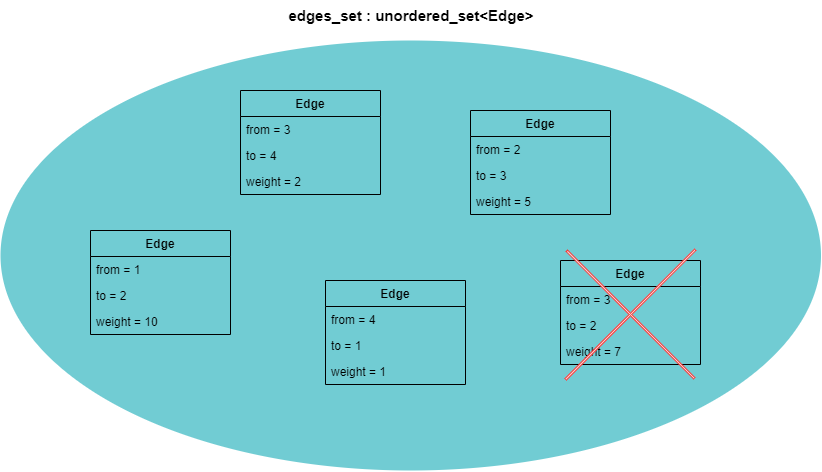
\includegraphics[width=0.7\textwidth]{./images/edges_setAbstract.png}
	\label{fig:edges_set}
\end{figure}

\begin{listing}[!hb]
\begin{minted}{c++}
// Shared/AdjacencyMapGraph.h
template <typename Label, typename Weight>
void add_edge(const Edge<Label, Weight> &edge) noexcept {
  const auto &[from, to, weight] = edge;
  vertex_weight_map_t &adj_map_from = adj_map[from];
  vertex_weight_map_t &adj_map_to = adj_map[to];

  // se l'arco in input esiste già, controlliamo il peso.
  // Se abbiamo già inserito un arco tra gli stessi nodi con un peso
  // maggiore, sovrascriviamo il vecchio arco con quello nuovo.
  if (adj_map_from.count(to)) {
    if (adj_map_from[to] > weight) {
      adj_map_from[to] = weight;
      adj_map_to[from] = weight;

      // rimuoviamo il vecchio arco con un peso più alto per aggiungere
      // lo stesso arco, ma con il nuovo peso più basso. Questo funziona
      // perché la funzione hash custom_hash::edge_hash, usata da
      // edge_set, è commutativa e non considera il campo "weight".
      edge_set.erase(edge);
      edge_set.insert(edge);
    }
  }
  // se l'arco in input è nuovo, lo aggiungiamo al grafo non diretto
  else {
    adj_map_from[to] = weight;
    adj_map_to[from] = weight;
    edge_set.insert(edge);
  }
}
\end{minted}
\caption{Implementazione del metodo \codeinline{add\_edge} di \textit{AdjacentMapGraph} che mette in evidenza l'impatto della funzione hash \codeinline{custom\_hash::edge\_hash}.}
\label{listing:add_edge}
\end{listing}

% L'ultimo problema non ancora affrontato riguarda la possibilità di inserire un arco doppio tra due nodi uguali (come richiesto da problema), con la differenza che questi due archi hanno un peso diverso. Siccome la nostra implementazione non prevede la presenza di tali archi doppi, la funzione \codeinline{add\_eddge()} si occupa di verificare l'eventuale presenza di un arco già inserito e di conseguenza i relativi pesi, per andare a modificare il peso qualora il peso del nuovo arco sia inferiore al peso dell'arco precedentemente già inserito. Per fare questo ad ogni aggiunta di un nuovo arco si va a verificare nella lista di adiacenza l'esistenza di un arco per quei due vertici:
% \begin{itemize}
% 	\item \textbf{se l'arco era già stato aggiunto:} si confrontano i due pesi e si aggiorna il peso dell'arco solo nell'eventualità in cui il nuovo peso sia inferiore a quello già presente nella lista di adiacenza. Dopodiché se c'è stato un aggiornamento si aggiorna anche il relativo \codeinline{unordered\_set}, eliminando l'arco precedente e si ri-aggiunge l'arco con il nuovo peso.
% 	\item \textbf{se l'arco non era già stato inserito:} si inserisce l'arco sia nella lista di adiacenza che in \codeinline{unordered\_set}.
% \end{itemize}

\noindent Le operazioni di inserimento nei container \codeinline{std::unordered\_map} e \codeinline{std::unordered\_set} hanno complessità temporale \complexityConstant{} ammortizzata. Dal momento che sappiamo a priori il numero di vertici da inserire in \codeinline{adj\_map} e il numero di archi da inserire in \codeinline{edge\_set}, abbiamo preallocato un numero di bucket sufficienti ad evitare costosi \textit{rehash} in entrambi i casi, rimuovendo di fatto il fattore ammortizzato.

\subsubsection {Costruzione del Grafo}

\textit{Shared/adjacency\_map\_graph\_factory.h} definisce una funzione di utilità che scorre tutte le righe del file in ingresso, salva gli archi in un vettore temporaneo, e lo trasferisce tramite \textit{move semantics} ad un nuovo oggetto di tipo \codeinline{AdjacencyMapGraph}. La mappa di adiacenza interpreta il grafo come spiegato nella sezione \ref{sub:graph-representation}. \\

\noindent \textbf{NOTA}: la label dei nodi di ogni grafo è decrementata di 1 in fase di lettura del dataset di input. Il grafo viene quindi rappresentato con nodi le cui label sono nel range $[0, n-1]$.
Questo semplifica e rende più leggibile l'implementazione di alcune strutture dati (ad esempio i Disjoint Set) e la costruzione dell'MST con Prim.

\subsection{Strutture Dati}

Tutte le strutture dati elencate di seguito sono definite nella cartella \textit{Shared}.
Ove possibile, per la nomenclatura dei metodi abbiamo cercato di seguire lo stesso standard dei container STL di C++.
Inoltre, le strutture dati usate sono sempre pre-allocate in memoria quando possibile, evitando rehashing e riallocazioni dispendiose. Questo significa che la maggior parte delle operazioni indicate con \complexityConstant{} ammortizzato siano in realtà totalmente costanti nella pratica.

\subsubsection{Heap}

\textit{Heap.h} contiene la definizione astratta di una generica Heap.
Gli elementi della Heap sono salvati in un \codeinline{std::vector}.
Per generalizzare il concetto di MinHeap/MaxHeap, la classe usa un comparatore binario booleano. Se il funtore dato in input alla classe è
\codeinline{std::greater<>}, la struttura dati avrà la semantica di una Min Heap; viceversa, con il comparatore \codeinline{std::less<>} si avrà la semantica di una Max Heap.

\paragraph{Ottimizzazioni}\mbox{} \\

\noindent Il parametro template \textit{IsAlreadyHeap} è usato per evitare di costruire la Heap se l'utente specifica che il container dato in input alla struttura dati rispetta già la proprietà di essere una Heap. Il controllo su questo flag booleano avviene a compile-time. Questa ottimizzazione garantisce un risparmio di tempo pari a \complexityN{}, ed è usata nell'implementazione dell'algoritmo di \textbf{Prim}. \\

\noindent I metodi che ripristinano la prioprietà di Heap (\codeinline{heapify\_up} e \codeinline{heapify\_down}) sono definiti in modo iterativo invece che ricorsivo, poiché i compilatori di C++17 non sono in grado di ottimizzare funzioni \textit{head-recursive}. I benchmark ci hanno confermato infatti che, in questo caso, l'implementazione iterativa è nettamente più veloce dell'implementazione ricorsiva.

\subsubsection{Binary Heap}

\textit{BinaryHeap.h} contiene una classe concreta che eredita \textit{Heap.h} e ne implementa i metodi virtuali. Definisce una Binary Heap, ovvero è possibile rappresentare gli elementi salvati come un albero binario completo (tranne eventualmente l'ultimo livello, che potrebbe non essere completo) che rispetta la proprietà di ordinamento delle Heap.

\paragraph{Ottimizzazioni}\mbox{} \\

\noindent L'operazione di divisione per 2, utilizzata ad esempio per determinare i figli sinistro e destro di un nodo nella Heap, è stata sostituita con l'operazione di shift binario.

\subsubsection{K-ary Heap}

\textit{KHeap.h} contiene una classe concreta che eredita \textit{Heap.h} e ne implementa i metodi virtuali. Definisce una K-ary Heap, ovvero è possibile rappresentare gli elementi salvati come un albero k-ario completo (tranne eventualmente l'ultimo livello, che potrebbe non essere completo) che rispetta la proprietà di ordinamento delle Heap.
\textit{K} è un parametro template che deve essere strettamente maggiore di due.

\subsubsection{Priority Queue}

\textit{PriorityQueue.h} è una classe concreta che eredita privatamente \textit{BinaryHeap.h} o \textit{KHeap.h}, a seconda del parametro template \textit{Heap}.
La semantica di PriorityQueue dipende dal comparatore passato al costruttore, che indica se si vuole usare una coda di priorità basata su Min Heap o su Max Heap. \\

\noindent PriorityQueue ha accesso diretto ai nodi salvati nella Heap, e usa due container associativi di tipo \codeinline{std::unordered\_map} per tenere traccia delle chiavi e degli indici posizionali di ogni elemento della Heap, permettendone la lettura e l'aggiornamento in tempo costante ammortizzato. \\

\noindent Rispetto ai costruttori delle varie classi Heap, PriorityQueue richiede non un comparatore, bensì una factory di comparatori. A tale factory è data in input una mappa che associa i valori degli elementi della Heap alle rispettive chiavi. Poiché tale input è passato per reference, il comparatore generato userà sempre la versione più aggiornata della mappa.

\noindent L'operazione di aggiornamento di una chiave richiede chiavi strettamente discendenti nel caso di una MinHeap, e chiavi strettamente crescenti nel caso di una MaxHeap. Abbiamo imposto questo vincolo per mantenere la complessità di \codeinline{update\_key} logaritmica anziché lineare (come sarebbe se avessimo usato il metodo \codeinline{build\_heap} indistintamente).

\paragraph{Ottimizzazioni}\mbox{} \\

\noindent Poichè istanziare una PriorityQueue così generica e flessibile è un'operazione non banale, abbiamo creato una serie di funzioni di utilità di facile comprensione da usare. Ad esempio, per creare una coda di priorità basata su una Min Heap binaria, esiste il metodo \codeinline{make\_min\_priority\_queue} (analogamente esiste \codeinline{make\_min\_k\_priority\_queue} per Min K-Heap).
L'utente finale della classe non deve preoccuparsi di inserire manualmente tutti i parametri template di tali funzioni, grazie alla \textit{type deduction} di C++17.

\subsubsection{Disjoint Set}

La classe base astratta in \textit{DisjointSetBase.h} definisce il contratto dei metodi \codeinline{find} e \codeinline{unite} (il nome comunemente usato per questa operazione, \textit{union}, è una parola chiave riservata in C++).
Gli elementi sono salvati in un container \codeinline{std::vector} chiamato \textbf{parents}, sotto l'assunzione che gli elementi siano solo numeri interi positivi distinti numerati da $0$ a $n-1$.
Avremmo potuto rilassare questo vincolo usando una struttura dati \codeinline{std::unordered\_map}, ma abbiamo preferito evitare perché i vettori sono molto più performanti nella pratica. \\

\noindent È possibile rappresentare graficamente i Disjoint-Set come alberi.
\mintinline{c++}{parents[i]} indicizza il padre del nodo $i$. Al momento dell'inizializzazione della classe, ogni nodo è settato come padre di se stesso, come mostrato in figura \ref{fig:disjoint-set-base-parents}.

\begin{figure}[htbp]
	\centering
	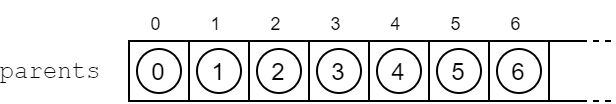
\includegraphics[width=0.7\textwidth]{./images/DisjointSetParentsVector.png}
	\caption{Inizializzazione di \codeinline{parents} nella classe \codeinline{DisjointSetBase}}
	\label{fig:disjoint-set-base-parents}
\end{figure}

\noindent Abbiamo realizzato due implementazioni diverse di Disjoint Set.
\codeinline{DisjointSet} adotta la policy \textit{union-by-size} vista a lezione, senza particolari ottimizzazioni. Definisce un membro \codeinline{std::vector} per salvare le dimensioni dei sottoalberi radicati nei vari nodi salvati, inizializzandolo a 1, come mostrato in figura \ref{fig:disjoint-set-sizes}.

\begin{figure}[htbp]
	\centering
    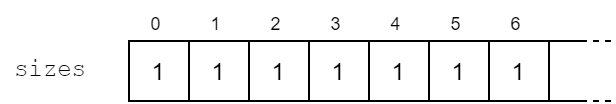
\includegraphics[width=0.7\textwidth]{./images/DisjointSetSizesVector.png}
	\caption{Inizializzazione di \codeinline{sizes} nella classe \codeinline{DisjointSet}}
	\label{fig:disjoint-set-sizes}
\end{figure}

\noindent \codeinline{DisjointSetCompressed}, invece, adotta la policy \textit{union-by-rank} con \textit{path-compression} tramite la tecnica \textit{path-splitting}.
Ad ogni invocazione del metodo \codeinline{find()} su un nodo $x$, ogni nodo nel percorso da $x$ all'antenato che identifica il set di $x$ è aggiornato per puntare al nodo ``nonno''. \\
\noindent DisjointSetCompressed definisce un membro \codeinline{std::vector} per salvare i rank dei vari nodi salvati, inizializzando il rank di ogni nodo a 0. Ad ogni invocazione del metodo \codeinline{unite()} su due nodi $x$ e $y$, ci sono due possibilità:

\begin{enumerate}
    \item \textbf{Gli alberi di $x$ e $y$ hanno lo stesso rank}: i rank del set che unirà $x$ e $y$ viene incrementato di 1;
    \item \textbf{Gli alberi di $x$ e $y$ hanno rank diversi}: il set che unirà $x$ e $y$ avrà rank pari a \\ $max\{ rank(find(x)), rank(find(y)) \}$.
\end{enumerate}

\noindent La \textit{path-compression} può modificare le altezze degli alberi ad ogni esecuzione, ma non cambierà mai il valore dei rank.
Nonostante sia possibile implementare tecniche di \textit{path-compression} anche con la policy \textit{union-by-size}, abbiamo deciso di cogliere l'opportunità di implementare la policy \textit{union-by-rank}, che non è stata spiegata a lezione. \\

\noindent In figura \ref{fig:disjoint-set-union-example} è possibile vedere un esempio di union-by-size implementato dalla classe \codeinline{DisjointSet}. Analogamente, in figura \ref{fig:disjoint-set-compressed-union-example} è possibile vedere un esempio di union-by-rank con path-splitting implementato dalla classe \codeinline{DisjointSetCompressed}.

\begin{figure}[h]
	\centering
	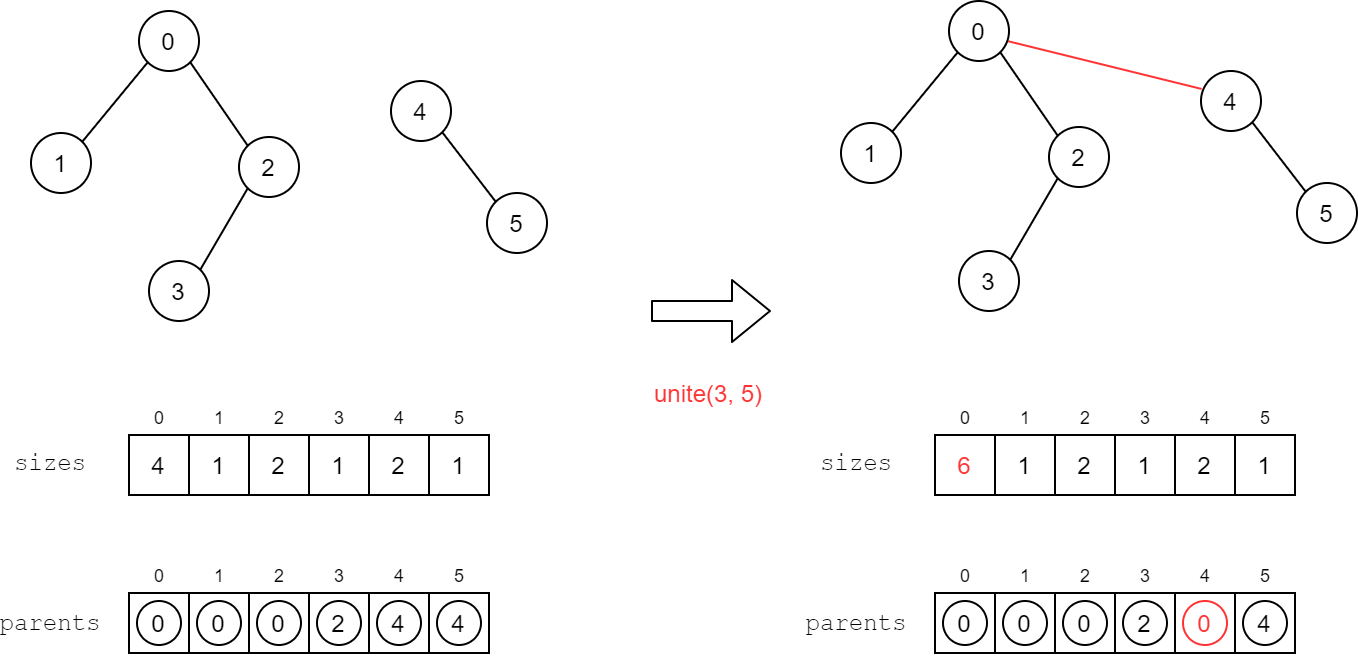
\includegraphics[width=0.9\textwidth]{./images/DisjointSetExample.png}
	\caption{Esempio di unione con DisjointSet}
	\label{fig:disjoint-set-union-example}
\end{figure}

\begin{figure}[h]
	\centering
	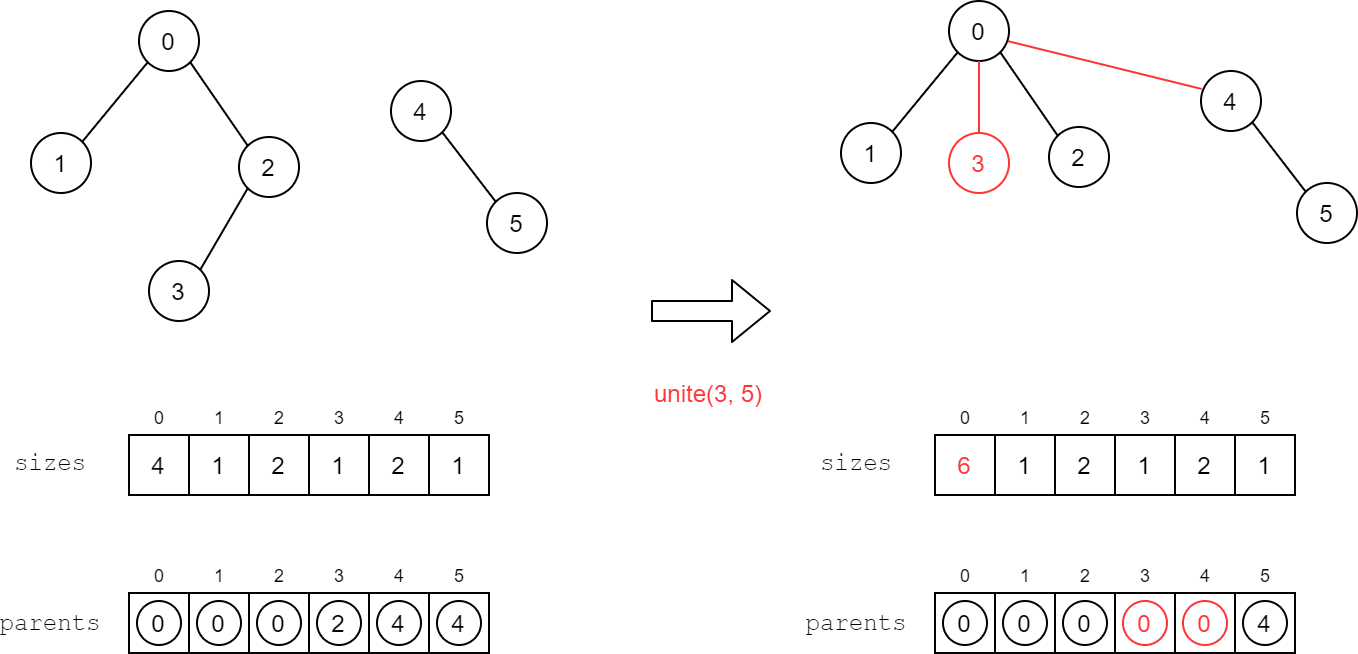
\includegraphics[width=0.9\textwidth]{./images/DisjointSetCompressedExample.png}
	\caption{Esempio di unione con DisjointSetCompressed}
	\label{fig:disjoint-set-compressed-union-example}
\end{figure}
